\documentclass{article}
\usepackage{amsmath}
\usepackage{amsthm}
\usepackage{amsfonts}
\usepackage{amssymb}
\usepackage{bbold}
\usepackage{dsfont}
\usepackage{graphicx}
\usepackage{cleveref}
\usepackage{bm}
\usepackage{booktabs}
\usepackage{siunitx}
\usepackage{xcolor}
\usepackage{pdfpages}
\usepackage[utf8]{inputenc}
\usepackage[english]{babel}
\newtheorem{definition}{Definition}
\newtheorem{example}{Example}
\newcommand{\exP}[1]{\mathrm{e}^{#1}}
\newcommand{\dif}{\mathrm{d}}
\renewcommand{\vec}[1]{\mathbf{#1}}
\newcommand{\pdagger}{{\phantom{\dagger}}}
\newcommand{\state}[1]{\vert #1\rangle}
\newcommand{\cstate}[1]{\langle #1\vert}
\newcommand{\tr}[1]{\mathrm{tr}\left\{#1\right\}}
\newcommand{\trs}[2]{\, \mathrm{tr}_{#1}\{#2\}}
\newcommand{\expc}[3]{\langle #1\vert #2 \vert #3\rangle}
\usepackage[doi=false,url=false,isbn=false,backend=bibtex,style=nature,natbib=true,sorting=none]{biblatex}
\bibliography{bib.bib}
\usepackage{geometry}
\geometry{
	a4paper,
	total={170mm,257mm},
	left=15mm,
	right=15mm,
	top=15mm,
}
\begin{document}
\title{TTHEOM in the Holstein model: Comparisons}
\maketitle

\section{Model}
The model is a junction, split into system, bath and interaction terms
\begin{equation}
	H = H_S + H_B + H_I
\end{equation}  
The system consists of a single electronic level with bare energy $\varepsilon_0$ coupled to a harmonic oscillator with frequency $\omega$, with Holstein-coupling $\lambda$
\begin{equation}
	H_S = \varepsilon_0 d^\dagger d + \omega a^\dagger a + \lambda d^\dagger d (a^\dagger + a).
\end{equation}
The bath are two electrodes $\ell=L,R$, modeled as free electrons
\begin{equation}
	H_B = \sum_{k\ell} \varepsilon_{k\ell}c^\dagger_{k\ell}c^\pdagger_{k\ell}
\end{equation}
and the system-bath coupling is linear in system and bath operators
\begin{equation}
	H = \sum_{k\ell} (V_{k\ell} c_{k\ell}^\dagger d + \mathrm{h.c.}).
\end{equation}
\section{Parameters}
The parameters of the model above are listed as follows
\begin{align*}
	\tilde{\varepsilon} &= \varepsilon_0 -\frac{\lambda^2}{\omega} = \SI{0.15}{\electronvolt}\\
	\omega &= \SI{0.2}{\electronvolt}\\
	\lambda &=0.2,0.3,\SI{0.4}{\electronvolt}\\ 
	\Gamma_\ell &= \SI{10}{\milli\electronvolt}\\
	T_\ell &= \SI{0.026}{\electronvolt}\\ 
	V &= 0,0.5,\SI{1}{\volt}\\
	W&=\mathrm{WBL}.
\end{align*}
\section{Results}
\begin{figure}[!h]
	\centering
	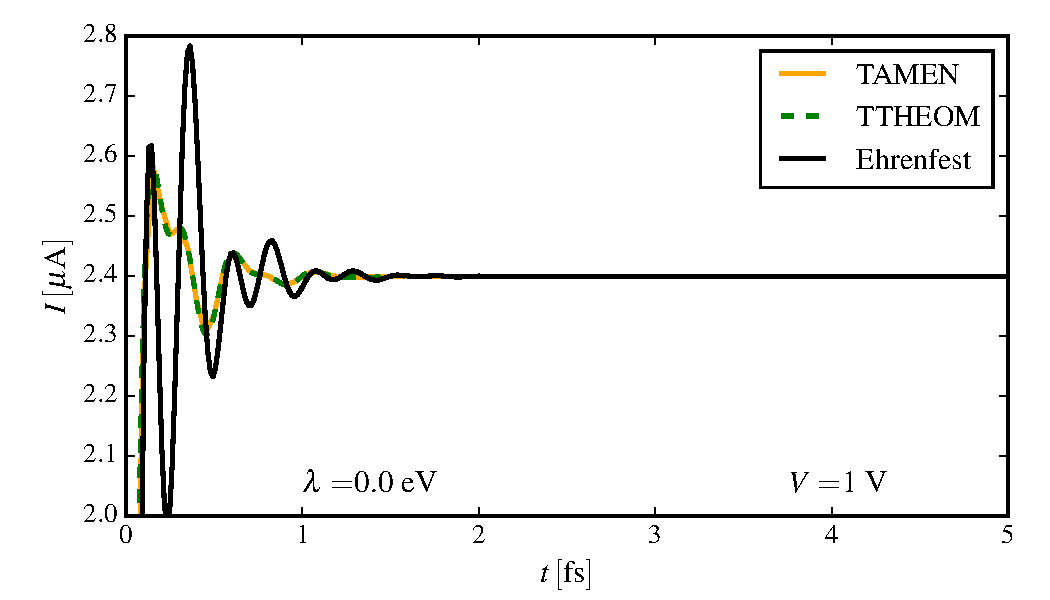
\includegraphics[width=0.8\textwidth]{figs/Holstein_lambda_0.0_VVar.pdf}
\end{figure}
\begin{figure}[!h]
	\centering
	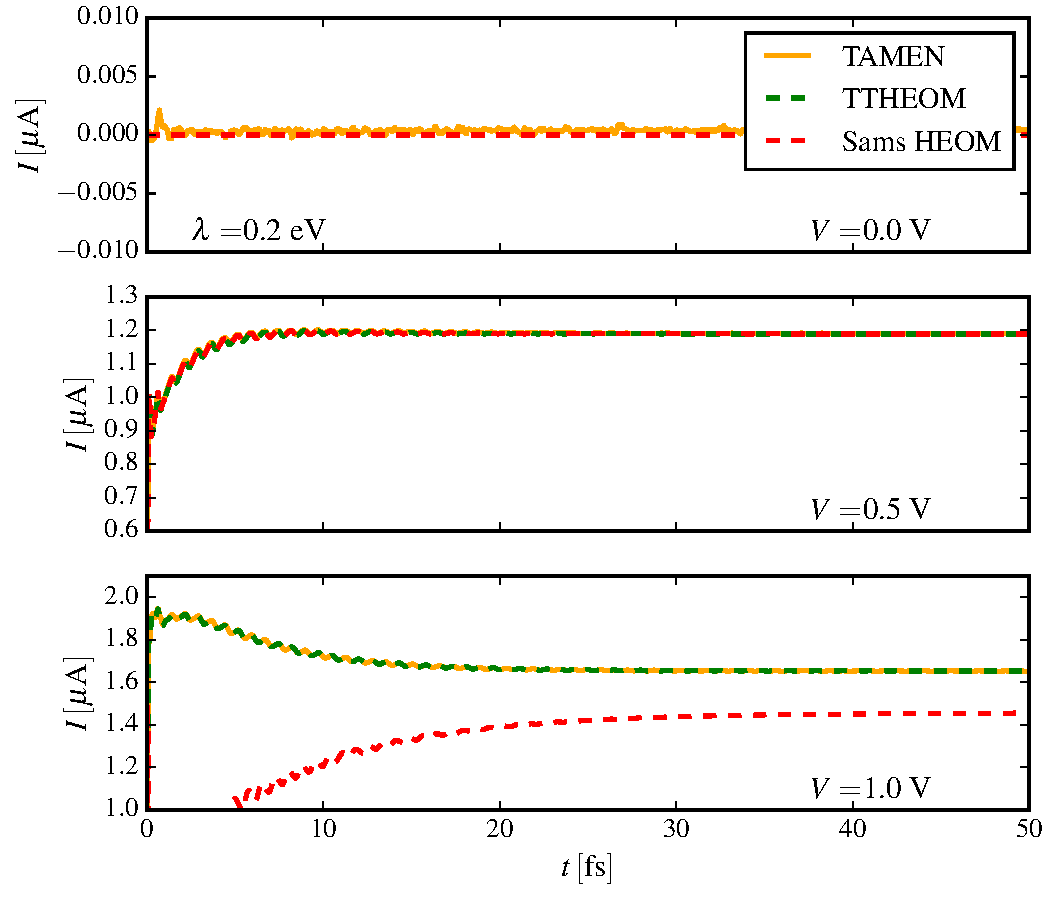
\includegraphics[width=0.8\textwidth]{figs/Holstein_lambda_0.2_VVar.pdf}
\end{figure}
\begin{figure}[!h]
	\centering
	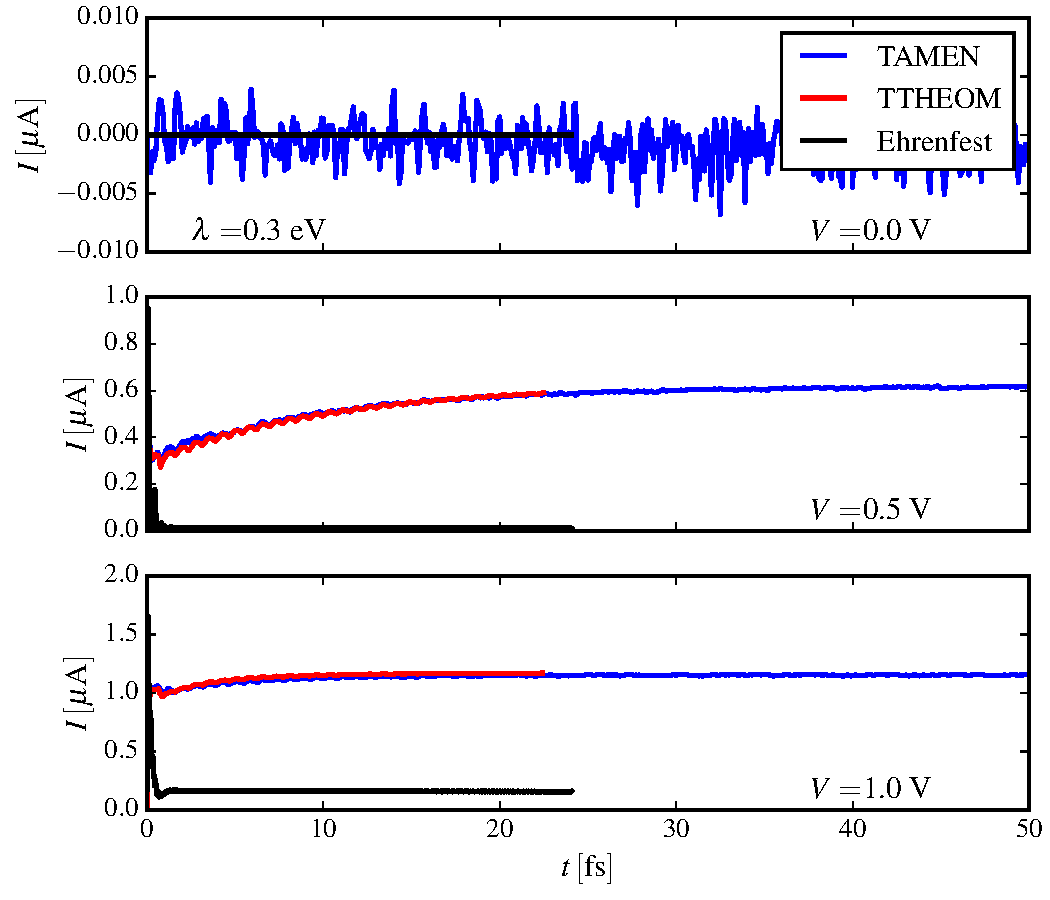
\includegraphics[width=0.8\textwidth]{figs/Holstein_lambda_0.3_VVar.pdf}
\end{figure}
\begin{figure}[!h]
	\centering
	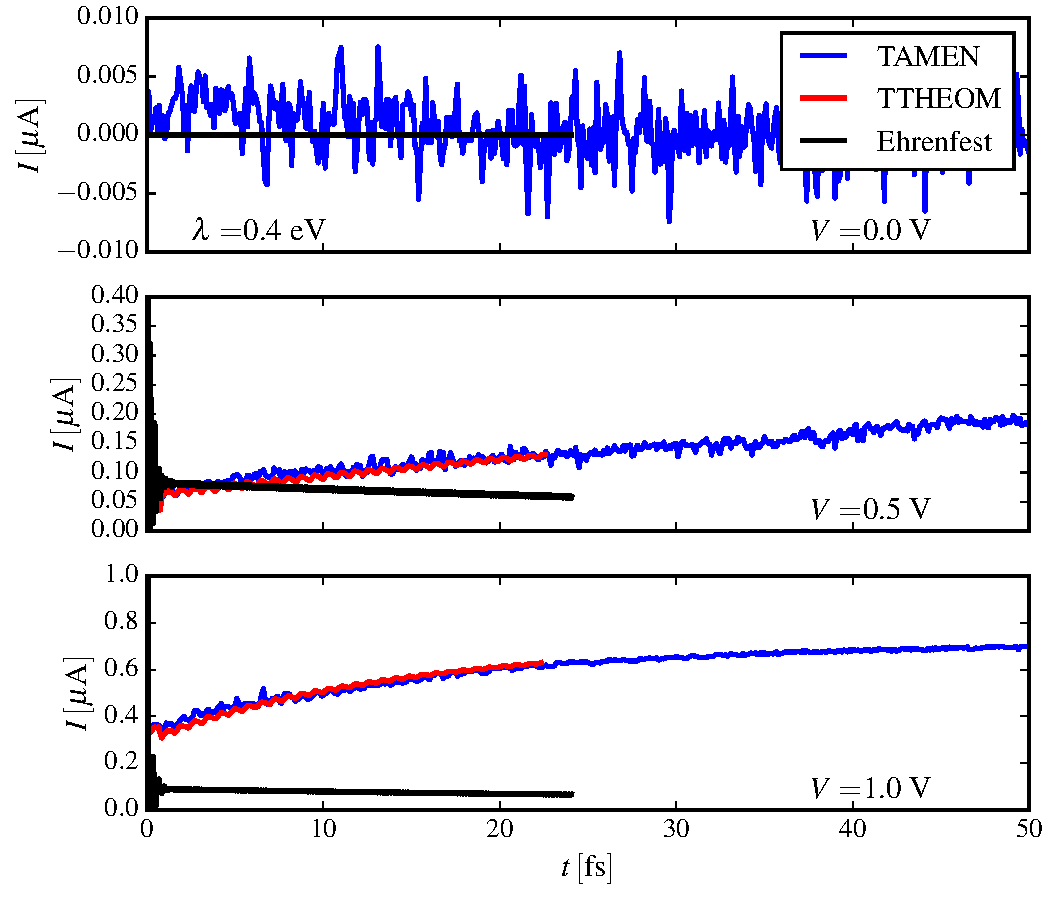
\includegraphics[width=0.8\textwidth]{figs/Holstein_lambda_0.4_VVar.pdf}
\end{figure}
\begin{figure}[!h]
	\centering
	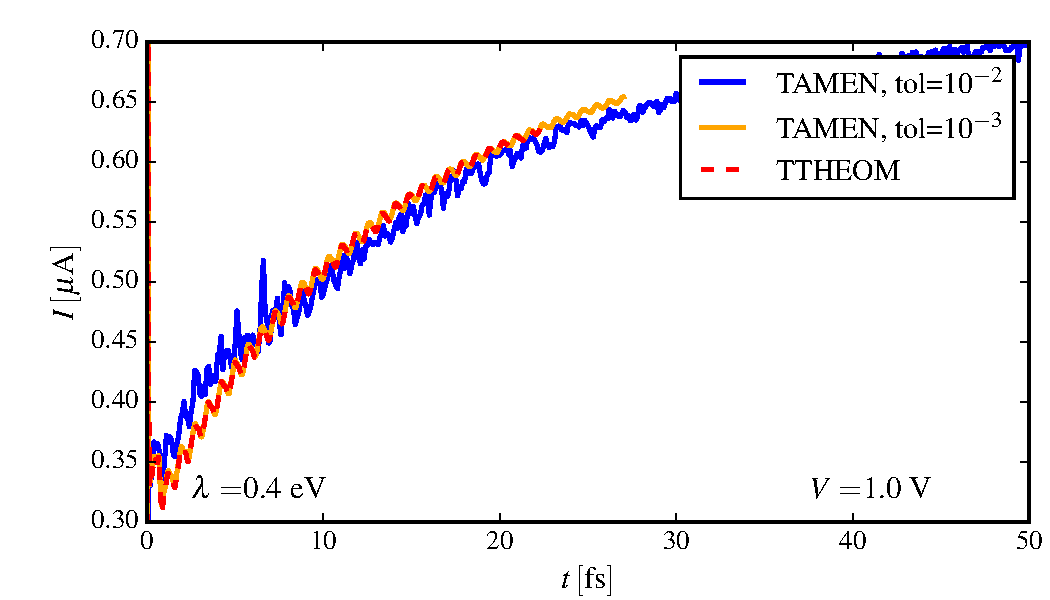
\includegraphics[width=0.8\textwidth]{figs/Holstein_lambda_0.4_V10_conv.pdf}
\end{figure}


\end{document}


